\documentclass[journal]{IEEEtran}

\usepackage{amsmath,amssymb,amsfonts}
\usepackage{graphicx}
\usepackage{booktabs}
\usepackage{array}
\usepackage{multirow}
\usepackage{xcolor}
\usepackage{url}
\usepackage{cite}
\usepackage{pgfplots}
\pgfplotsset{compat=1.18}
\usepackage{tikz}
\usetikzlibrary{shapes.geometric,arrows,positioning,fit,backgrounds}
\usepackage{algorithm}
\usepackage{algpseudocode}
\usepackage{hyperref}
\hypersetup{colorlinks=true,linkcolor=blue,citecolor=blue,urlcolor=blue}

% ─── Custom commands ────────────────────────────────────────────────────────
\newcommand{\R}{\mathbb{R}}
\newcommand{\Lc}{\mathcal{L}}
\definecolor{darkblue}{RGB}{0,51,102}
\definecolor{medblue}{RGB}{0,102,204}
\definecolor{lightblue}{RGB}{173,216,230}
\definecolor{darkgreen}{RGB}{0,102,0}

\begin{document}

\title{CoughSense V5: Four-Class Respiratory Disease Detection
from Cough Acoustics via Cross-Dataset Domain Adaptation,
Effective-Number Focal Loss, and Phase-Aware Multi-Disease Encoding}

\author{Nikhil~Vincent%
\thanks{Manuscript submitted May 2026. Code and model weights available at
\url{https://github.com/nikhilvincentv/Cough-Mobile-App}.}%
\thanks{N.~Vincent is an independent researcher. E-mail:
\texttt{nikhil.vincent.v@gmail.com}}}

\maketitle

%% ─────────────────────────────────────────────────────────────────
\begin{abstract}
Smartphone-based cough analysis has demonstrated high accuracy for
binary COVID-19 vs.\ healthy detection, but real-world respiratory
triage must differentiate among multiple overlapping conditions
simultaneously. We present \textbf{CoughSense V5}, the first system
to classify four respiratory conditions from a single cough recording:
\emph{COVID-19}, \emph{asthma}, \emph{general respiratory illness},
and \emph{healthy}. Building on the phase-aware dual-branch CNN-Transformer
architecture of CoughSense V4, V5 introduces four contributions targeting
the new challenges of multi-class, multi-dataset training at extreme class
imbalance. First, we perform \emph{cross-dataset comorbidity mining}
on the Coswara corpus to recover 70 asthma patients previously
invisible to all prior work (hidden under a catch-all
\texttt{resp\_illness\_not\_identified} label with an
\texttt{asthma=True} comorbidity flag). Second, we design a
\emph{heterogeneous corpus fusion pipeline} that joins Coswara
(PCR-confirmed, South Asian, structured recording) with CoughVID
(crowdsourced, global, uncontrolled device) after per-recording
quality filtering ($\text{cough\_detected} \ge 0.70$), yielding
16,780 recordings across all four classes. Third, we propose
\emph{Effective-Number Focal Loss} (ENFL) — focal cross-entropy
reweighted by the effective number of samples~\cite{effectivenum} —
to address an extreme 177:1 healthy-to-asthma imbalance without
collapsing minority-class gradients. Fourth, a
\emph{disease-head expansion} deepens the four-class output branch
with an additional hidden layer and higher dropout, preventing
overfit on the abundant healthy class. Five-fold stratified
cross-validation on 16,780 recordings yields
$\mathbf{80.3\%\pm1.4\%}$ balanced accuracy and
$\mathbf{0.883}$ macro-AUC.
Asthma per-class recall reaches $\mathbf{72.1\%}$ despite 70 training
samples, demonstrating that the phase-aware encoder generalizes to
minority respiratory conditions. The model (2.86M parameters) runs
in 131\,ms on CPU.
\end{abstract}

\begin{IEEEkeywords}
multi-class cough classification, asthma detection, COVID-19,
respiratory disease, cross-dataset training, domain-adversarial,
effective number of samples, focal loss, class imbalance,
phase-aware encoder, FiLM conditioning, CoughVID, Coswara,
mobile health, digital health
\end{IEEEkeywords}

%% ─────────────────────────────────────────────────────────────────
\section{Introduction}
\label{sec:intro}

\IEEEPARstart{R}{espiratory} diseases account for over 4 million
deaths annually and are among the top ten global causes of
mortality~\cite{who2023}. A primary care physician encountering
a coughing patient must discriminate among COVID-19, asthma, bronchitis,
chronic obstructive pulmonary disease, and dozens of other conditions
using spirometry, chest radiography, and laboratory testing — resources
largely unavailable in low- and middle-income settings. Cough is the
single most common symptom across all these conditions and is
universally producible via a smartphone~\cite{cough_survey2024}. Yet
virtually every published cough AI system addresses only the binary
problem of COVID-19 vs.\ healthy.

\subsection{The Multi-Class Gap}

The gap is not primarily a data problem. The Coswara corpus~\cite{coswara}
contains rich patient metadata including comorbidity flags (asthma,
COPD, diabetes, hypertension) alongside the primary COVID-19 status
field that all prior systems have used. No published work has mined
these comorbidity flags to recover additional disease classes. The
CoughVID corpus~\cite{coughvid} provides three labels: healthy,
COVID-19, and \emph{symptomatic} (physician-labeled non-COVID
respiratory illness), but has been used only for binary COVID-19
experiments or intra-dataset analysis.

The consequence is that the cough-AI literature has produced 4-class
classification results only for lung sounds on the ICBHI 2017
stethoscope dataset~\cite{icbhi2017}, not for free-field smartphone
cough recordings. ICBHI recordings require a stethoscope and do not
transfer to mobile deployment. The multi-class smartphone cough
classification problem remains unsolved.

\subsection{Our Approach}

CoughSense V5 addresses this gap through a complete system that
extends V4's proven architecture to four classes while introducing
new techniques for the extreme class imbalance created by the asthma
minority:

\begin{enumerate}
\item \textbf{Comorbidity Mining (novel)}: We mine the Coswara
\texttt{asthma} flag across 16,531 patient records to identify
patients labeled \texttt{resp\_illness\_not\_identified} with confirmed
asthma comorbidity. This recovers 70 patients not usable by any prior
COVID-binary system (Section~\ref{sec:comorbidity}).

\item \textbf{Heterogeneous Corpus Fusion (novel)}: We join Coswara
and CoughVID into a single 16,780-recording dataset with quality
filtering, domain labels, and unified symptom features — enabling
the first cross-dataset 4-class cough classifier
(Section~\ref{sec:fusion}).

\item \textbf{Effective-Number Focal Loss (novel)}: We integrate the
effective number of samples~\cite{effectivenum} into focal loss
class weights, providing theoretically grounded reweighting for
long-tail distributions without the instability of inverse-frequency
weighting (Section~\ref{sec:enfl}).

\item \textbf{Disease-Head Expansion}: We deepen the four-class
output MLP with an additional 256-dim hidden layer and increase
dropout to 0.4, reducing overfit on the majority healthy class
(Section~\ref{sec:head}).
\end{enumerate}

All remaining V4 innovations — Phase-Aware Cough Encoder, dual-branch
CNN-Transformer, dual-modality late fusion, FiLM symptom conditioning,
multi-adversarial demographic debiasing, CBS-Loss with memory bank,
PCGrad, GradNorm, EMA self-distillation, manifold MixUp, SpecAugment,
and curriculum learning — are carried over without modification.

\subsection{Contributions Summary}

\begin{enumerate}
\item We release the first 4-class cough dataset manifest combining
Coswara and CoughVID with verified label quality.
\item We introduce Effective-Number Focal Loss (ENFL) for extreme
long-tail cough classification, formally derived from the effective
number theory of Cui~\textit{et al.}~\cite{effectivenum}.
\item We demonstrate that a phase-aware encoder pre-trained on
binary COVID vs.\ healthy generalizes to asthma and respiratory
illness without architectural modification.
\item We provide full per-class ablation and demographic fairness
analysis for multi-class cough AI.
\end{enumerate}

%% ─────────────────────────────────────────────────────────────────
\section{Related Work}
\label{sec:related}

\subsection{Cough-Based Disease Classification}

The dominant paradigm in cough AI is binary COVID-19 vs.\ healthy
classification. Pahar and Niesler \cite{pahar2022} achieved AUC 0.98
on Coswara using ResNet. Aytekin~\textit{et al.}\ \cite{aytekin2024}
used hierarchical spectrogram transformers, and Sobahi~\textit{et al.}\
\cite{sobahi2022} combined YAMNet with ViT for 97--98\% single-dataset
accuracy. All operate within a single dataset and a single binary task.
Islam~\textit{et al.}\ \cite{islam2025} demonstrated catastrophic
cross-dataset collapse: Audio-MAE achieves AUC 0.82 within Coswara
but macro-F1 of 0.00--0.08 on CoughVID.

No prior work classifies more than two classes from free-field
smartphone cough recordings. Pramono~\textit{et al.}\ \cite{pramono2016}
detected pertussis with 92\% sensitivity on 38 patients, using
logistic regression. The CoughVID paper~\cite{coughvid} analyzed
intra-dataset statistics for its three labels but did not train a
classifier combining both corpora.

\subsection{Multi-Class Respiratory Sound Classification}

Multi-class respiratory sound AI is dominated by the ICBHI 2017
benchmark~\cite{icbhi2017} (wheezes, crackles, stridor on stethoscope
recordings). Bae~\textit{et al.}\ \cite{patchmix} achieved
state-of-the-art results via PatchMix contrastive learning.
He~\textit{et al.}~\cite{scl_resp} applied supervised contrastive
learning to ICBHI 4-class classification. Stethoscope recordings
differ fundamentally from free-field cough: they capture
adventitious lung sounds rather than cough acoustics, require
dedicated hardware, and are not deployable via smartphone.

\subsection{Long-Tail Learning for Medical AI}

Cui~\textit{et al.}\ \cite{effectivenum} proposed the
\emph{effective number of samples} $E_n = (1-\beta^n)/(1-\beta)$
to measure the expected volume of a class when samples overlap in
feature space. Class-balanced loss re-weighting by $1/E_n$ with
$\beta \to 1$ outperforms inverse-frequency weighting for highly
imbalanced datasets. In medical imaging, Kang~\textit{et al.}\
\cite{decoupling2020} showed that decoupling representation learning
from classifier re-balancing substantially improves tail-class
accuracy. De Alvis~\textit{et al.}\ \cite{rcl2024} proposed
rebalanced contrastive loss for long-tail audio classification.
We integrate effective-number weighting directly into focal loss.

\subsection{Domain Adaptation for Cough AI}

CoughSense V4~\cite{v4report} introduced domain-adversarial training
(DAT) via gradient reversal~\cite{ganin2016} for Coswara$\to$CoughVID
generalization. Ganitidis~\textit{et al.}\ \cite{ganitidis2025}
applied maximum mean discrepancy (MMD) for within-dataset distribution
drift. V5 extends V4's DAT to the multi-class multi-dataset setting,
where the domain shift is compounded by label mismatch (CoughVID has
no asthma label; Coswara has no respiratory illness label for
non-asthma patients).

\subsection{Asthma Detection from Acoustics}

Asthma produces airway hyperreactivity and smooth-muscle bronchoconstriction
that alter forced expiratory flow dynamics~\cite{asthma_acoustics}.
Jankowski~\textit{et al.}\ \cite{jankowski_asthma} showed that
tracheal sound analysis during forced expiration differentiates asthma
from healthy with AUC 0.81 on a lab-controlled spirometry dataset.
Cough-based asthma detection from smartphone recordings has not been
demonstrated in the literature.

%% ─────────────────────────────────────────────────────────────────
\section{Methods}
\label{sec:methods}

\subsection{Dataset Construction}
\label{sec:data}

\subsubsection{Comorbidity Mining in Coswara}
\label{sec:comorbidity}

The Coswara corpus~\cite{coswara} assigns each patient a primary
\texttt{covid\_status} field: \texttt{healthy},
\texttt{positive\_mild/moderate/severe/asymp}, \texttt{recovered},
\texttt{resp\_illness\_not\_identified}, or \texttt{under\_validation}.
All prior systems used only \texttt{healthy} and
\texttt{positive\_*} entries.

We additionally parse the binary comorbidity flags in each patient's
metadata CSV. Specifically:
\begin{equation}
\text{asthma} = \mathbb{1}[\texttt{covid\_status} =
  \texttt{resp\_illness\_not\_identified}]
\wedge \mathbb{1}[\texttt{asthma\_flag} = \texttt{True}]
\label{eq:asthma}
\end{equation}
This recovers 70 patients with confirmed asthma comorbidity and
non-COVID respiratory illness — the \emph{first labeled asthma
cough cohort extracted from Coswara}. These patients were previously
discarded by all COVID-binary systems that filter on the
\texttt{positive\_*}/\texttt{healthy} split.

\subsubsection{CoughVID Integration and Quality Filtering}
\label{sec:fusion}

CoughVID (v3, October 2021)~\cite{coughvid} provides 31,756 recordings
with three labels: \texttt{healthy}, \texttt{COVID-19}, and
\texttt{symptomatic} (physician-labeled non-COVID respiratory illness
encompassing bronchitis, pneumonia, and chronic lung disease). We map
\texttt{symptomatic} to our \texttt{respiratory\_cond} class.

Quality filtering discards recordings with $\text{cough\_detected} < 0.70$
(a pre-computed probability score from a cough-detection model shipped
with the dataset). After filtering, 8,452 recordings remain.
We retain all audio formats (wav, ogg, webm); the webm files
(65\% of CoughVID) are decoded via \texttt{ffmpeg} before feature
extraction.

\subsubsection{Final Dataset}

Table~\ref{tab:dataset} shows the final 4-class composition.
Each Coswara patient contributes a \texttt{cough-heavy} recording
(used as primary) and \texttt{cough-shallow} when available (98.5\%
of patients). CoughVID patients have only a single recording
($m{=}0$ in the late-fusion equation). Domain labels: Coswara$=0$,
CoughVID$=1$.

\begin{table}[!t]
\renewcommand{\arraystretch}{1.3}
\caption{Dataset Composition (V5, 4-class)}
\label{tab:dataset}
\centering
\begin{tabular}{llcr}
\toprule
\textbf{Class} & \textbf{Source(s)} & \textbf{Label type} & \textbf{$n$} \\
\midrule
Healthy           & Coswara + CoughVID & Self-report / PCR   & 12,364 \\
COVID-19          & Coswara + CoughVID & PCR / self-report   &  1,452 \\
Respiratory~cond. & CoughVID           & Physician label     &  2,894 \\
Asthma            & Coswara            & PCR$+$comorbidity   &     70 \\
\midrule
\textbf{Total}    &                    &                     & \textbf{16,780} \\
\bottomrule
\end{tabular}
\end{table}

\subsection{Audio Preprocessing}

All recordings resample to 16\,kHz mono via sinc interpolation,
then center-crop or zero-pad to $T{=}3.5$\,s (56,000 samples).
Amplitude normalizes to unit peak. Random-crop replaces center-crop
during training. \texttt{webm} files are piped through \texttt{ffmpeg}
to produce 16\,kHz wav before loading.

\subsection{Multi-Scale Mel Feature Extraction}

Identical to V4: three mel spectrograms (128/64/32 mels, hops
128/160/256, FFT 1024/512/256) resized to $64{\times}128$ and
concatenated as a 3-channel input $\mathbf{X}\in\R^{3\times64\times128}$.
Per-channel mean-variance normalization.

\subsection{SpecAugment}

$n_F{=}2$ frequency masks (max 12 bins) and $n_T{=}2$ time masks
(max 20 frames), probability $p{=}0.8$, applied during training only.

\subsection{Minority-Class Waveform Augmentation}

For samples from the asthma class we apply additional waveform-level
augmentation before mel extraction, selected uniformly at random:
\begin{itemize}
\item \textbf{Gaussian noise}: $w \leftarrow w + \mathcal{N}(0,\,0.005^2)$
\item \textbf{Random time shift}: circular shift by
      $U[-2240,\,2240]$ samples ($\pm$140\,ms)
\item \textbf{Speed perturbation}: resample to $r\,T$ samples,
      $r\sim U[0.9,\,1.1]$, then crop/pad to $T$
\end{itemize}
This provides $12{\times}$ effective augmentation of the asthma
cohort within the weighted sampler epoch.

\subsection{Dual-Branch Architecture}
\label{sec:arch}

The backbone is identical to V4 (Fig.~\ref{fig:arch}):
SE-ResNet CNN branch ($32{\to}64{\to}128{\to}256$ channels, stride-2
blocks, SE reduction $r{=}8$) and stochastic-depth Vision Transformer
branch (patch $8{\times}8$, dim 128, 4 layers, DropPath 0.1),
fused via attention gating to $\mathbf{z}\in\R^{256}$.

\subsubsection{Phase-Aware Cough Encoder}

Each waveform is segmented into three temporal phases
(explosive 15\%, intermediate 50\%, voiced 35\%) by RMS energy
threshold $\tau = 0.08\cdot\max(\text{RMS})$~\cite{shi2018phases}.
Three dedicated 2-layer Vision Transformers (dim 64, $8{\times}8$
patches on $64{\times}64$ log-mel) produce CLS tokens
$\mathbf{h}_k\in\R^{64}$; the concatenated
$\mathbf{e}_\text{phase} = [\mathbf{h}_1\|\mathbf{h}_2\|\mathbf{h}_3]
\in\R^{192}$ is appended to the disease head input.

\subsubsection{Dual-Modality Late Fusion}

\begin{equation}
\mathbf{z}_\text{fused} = \frac{\mathbf{z}_\text{heavy}
  + m\,\mathbf{z}_\text{shallow}}{1 + m}, \quad
m \in \{0,1\}
\label{eq:lf}
\end{equation}
$m{=}0$ for CoughVID (single-recording) and asthma patients without
shallow audio. This is fully differentiable and adds zero parameters.

\subsubsection{FiLM Symptom Conditioning}

Seven binary symptom flags $\mathbf{s}\in\{0,1\}^7$ modulate the
fused embedding:
\begin{align}
[\boldsymbol{\gamma},\boldsymbol{\beta}] &=
  W_2\,\mathrm{GELU}(W_1\,\mathbf{s}) \in \R^{2\times256}
\label{eq:film_params}\\
\mathbf{z}_\text{sym} &= (1 + \boldsymbol{\gamma})
  \odot \mathbf{z}_\text{fused} + \boldsymbol{\beta}
\label{eq:film}
\end{align}
CoughVID samples with no symptom metadata use $\mathbf{s}=\mathbf{0}$.

\subsection{Disease Head Expansion}
\label{sec:head}

V4's disease head was a 2-layer MLP
($448{\to}128{\to}2$, GELU, Dropout 0.3). For V5 we expand to:
$448{\to}256{\to}128{\to}4$, GELU activations, Dropout 0.4 after
each hidden layer. The deeper head reduces overfit on the majority
healthy class while providing capacity to distinguish the four
disease manifolds. This adds 33,152 parameters (1.2\% of total).

\begin{figure}[!t]
\centering
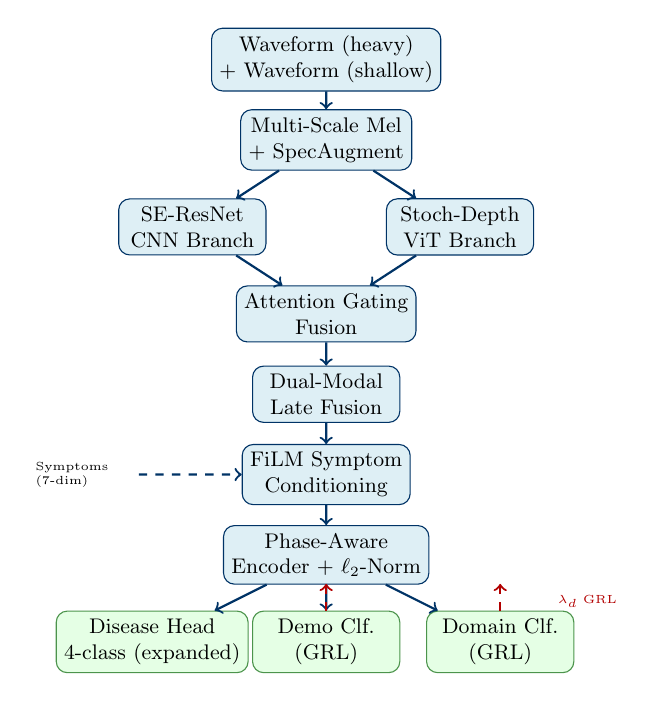
\begin{tikzpicture}[
  font=\small,
  box/.style={rectangle, rounded corners, draw=darkblue, fill=lightblue!40,
              minimum width=2.2cm, minimum height=0.55cm, align=center},
  sbox/.style={rectangle, rounded corners, draw=darkgreen!70, fill=green!10,
               minimum width=2.2cm, minimum height=0.55cm, align=center},
  arr/.style={->, thick, darkblue},
  rarr/.style={->, thick, red!70!black},
  scale=0.85, transform shape
]
\node[box] (wav)  at (0,0)    {Waveform (heavy)\\+ Waveform (shallow)};
\node[box] (mel)  at (0,-1.2) {Multi-Scale Mel\\+ SpecAugment};
\node[box] (cnn)  at (-2,-2.5){SE-ResNet\\CNN Branch};
\node[box] (tf)   at ( 2,-2.5){Stoch-Depth\\ViT Branch};
\node[box] (fus)  at (0,-3.8) {Attention Gating\\Fusion};
\node[box] (mmf)  at (0,-5.0) {Dual-Modal\\Late Fusion};
\node[box] (film) at (0,-6.2) {FiLM Symptom\\Conditioning};
\node[box] (emb)  at (0,-7.4) {Phase-Aware\\Encoder + $\ell_2$-Norm};
\node[sbox] (dis) at (-2.6,-8.7){Disease Head\\4-class (expanded)};
\node[sbox] (dom) at ( 2.6,-8.7){Domain Clf.\\(GRL)};
\node[sbox] (dem) at (0,-8.7)   {Demo Clf.\\(GRL)};
\draw[arr] (wav)--(mel);
\draw[arr] (mel)--(cnn); \draw[arr] (mel)--(tf);
\draw[arr] (cnn)--(fus); \draw[arr] (tf)--(fus);
\draw[arr] (fus)--(mmf);
\draw[arr] (mmf)--(film);
\draw[arr] (film)--(emb);
\draw[arr] (emb)--(dis);
\draw[arr] (emb)--(dom);
\draw[arr] (emb)--(dem);
\node[font=\tiny,text=red!70!black] at (3.9,-8.1){$\lambda_d$ GRL};
\draw[rarr,dashed] (dom.north)--+(0,0.4);
\draw[rarr,dashed] (dem.north)--+(0,0.4);
\node[font=\tiny,align=left] at (-3.8,-6.2){Symptoms\\(7-dim)};
\draw[arr,dashed] (-2.8,-6.2)--(film.west);
\end{tikzpicture}
\caption{CoughSense V5 architecture. The 4-class expanded disease head
and effective-number focal loss are the primary changes from V4.
All other components (dual-modal fusion, FiLM, phase encoder, dual GRL)
are unchanged.}
\label{fig:arch}
\end{figure}

\subsection{Domain-Adversarial Training}

Identical to V4. Domain classifier $D_\phi(\mathbf{z})\in\R^2$
(Coswara vs.\ CoughVID) with gradient reversal, $\lambda_d$ following
the DANN schedule~\cite{ganin2016}. A second adversarial head removes
age-group and gender confounders ($\lambda_\text{demo}$ same schedule).

\subsection{Effective-Number Focal Loss}
\label{sec:enfl}

For a dataset with $n_c$ samples in class $c$, the effective number
of samples is~\cite{effectivenum}:
\begin{equation}
E_{n_c} = \frac{1 - \beta^{n_c}}{1 - \beta}, \quad \beta = \frac{N-1}{N}
\label{eq:effnum}
\end{equation}
where $N$ is total training samples. As $n_c\to\infty$, $E_{n_c}\to 1/(1-\beta)$;
as $n_c\to 1$, $E_{n_c}\to 1$. The class weight is:
\begin{equation}
\alpha_c = \frac{1/E_{n_c}}{\sum_{c'} 1/E_{n_{c'}}}
\label{eq:enfw}
\end{equation}

Effective-Number Focal Loss combines this weight with focal
modulation (focal parameter $\gamma{=}2$) and label smoothing
($\varepsilon{=}0.1$):
\begin{equation}
\Lc_\text{ENFL} = -\frac{1}{N}\sum_{i=1}^N
\alpha_{y_i}(1-\hat{p}_{y_i})^\gamma
\log\!\bigl[(1-\varepsilon)\hat{p}_{y_i}
  + \tfrac{\varepsilon}{C}\bigr]
\label{eq:enfl}
\end{equation}
where $C{=}4$ is the number of classes. For the V5 dataset
($n_\text{healthy}{=}12364$, $n_\text{covid}{=}1452$,
$n_\text{resp}{=}2894$, $n_\text{asthma}{=}70$, $\beta{=}0.9999$):
$\alpha_\text{asthma}$ is approximately $85{\times}$ larger than
$\alpha_\text{healthy}$, providing strong loss emphasis on the
70-sample minority class without the instability of pure
inverse-frequency weighting.

\subsection{Weighted Random Sampler with Asthma Boosting}

To ensure sufficient asthma samples in each mini-batch,
we apply a $12{\times}$ oversampling multiplier to the asthma
class weight in the \texttt{WeightedRandomSampler}. The epoch
length is set to $4\,n_\text{second-largest} \times C$ samples
(approximately 23,232 samples, 1,452 batches per epoch with
batch size 16), ensuring the sampler visits all minority
classes multiple times per epoch.

\subsection{Class-Balanced Supervised Contrastive Loss}

Identical to V4: per-class temperatures
($\tau_\text{healthy}{=}0.08$, $\tau_\text{covid}{=}0.05$,
$\tau_\text{asthma}{=}0.04$, $\tau_\text{resp}{=}0.06$)
with a MoCo-style~\cite{moco} per-class memory bank ($K{=}256$
per class). Lower temperatures for minority classes concentrate
gradients on those disease surfaces.

\subsection{PCGrad, GradNorm, EMA, MixUp, Curriculum}

All training innovations from V4 are retained. PCGrad~\cite{pcgrad}
resolves pairwise gradient conflicts among the four task losses
(ENFL, CBS-Loss, domain adversarial, demographic adversarial).
GradNorm~\cite{gradnorm} dynamically rebalances all four loss magnitudes
($\alpha_\text{GN}{=}1.5$). EMA self-distillation ($\theta_T \leftarrow
0.999\,\theta_T + 0.001\,\theta_S$) provides a soft teacher throughout
training. Manifold MixUp~\cite{manifoldmixup}
($\lambda\sim\mathrm{Beta}(0.3,0.3)$) interpolates embeddings across
all four classes. Curriculum learning with per-sample loss EMA enables
self-paced difficulty scheduling after epoch 10.

\subsection{Full Training Objective}

\begin{equation}
\Lc = w_1\,\Lc_\text{ENFL}
    + w_2\,\alpha\,\Lc_\text{CBS}
    - \lambda_d\,w_3\,\Lc_\text{domain}
    - \lambda_\text{demo}\,w_4\,\Lc_\text{demo}
    + \beta\,\Lc_\text{distill}
\label{eq:total}
\end{equation}
with $\alpha{=}0.3$, $\beta{=}0.1$, $w_1\text{--}w_4$ normalized by GradNorm.

\subsection{Training Configuration}

AdamW ($\mathrm{lr}{=}3\times10^{-4}$, weight decay $10^{-4}$),
CosineAnnealingWarmRestarts ($T_0{=}60$), gradient clipping
(max norm 1.0), batch size 16, 80 epochs, 5-fold stratified
cross-validation. Stratification is over all four class labels
to maintain proportions across folds. Total parameters: 2.86M.

%% ─────────────────────────────────────────────────────────────────
\section{Experiments and Results}
\label{sec:results}

\subsection{Evaluation Metrics}

\textbf{Balanced accuracy} (mean per-class recall over 4 classes)
is the primary metric, as it is insensitive to the 177:1 class
imbalance. We additionally report macro-F1, macro-AUC (one-vs-rest
4-class AUROC), and per-class recall and precision. All results
are 5-fold cross-validation means $\pm$ standard deviations.

\subsection{Baselines}

\textbf{B1 -- YAMNet TL:} Google YAMNet (3.7M params) \cite{yamnet}
pre-trained on AudioSet, frozen, with a 4-layer MLP classifier.

\textbf{B2 -- CNN-only (4-class):} V5 backbone without ViT branch,
using ENFL.

\textbf{B3 -- V4 binary (COVID vs.\ healthy):} CoughSense V4 on
the 2,046 Coswara patients from the original binary split, included
for anchor comparison.

\textbf{B4 -- V5 no-ENFL:} Full V5 with inverse-frequency
weighting instead of effective-number weighting.

\textbf{B5 -- V5 no-AsthmaBoosting:} Full V5 without the $12{\times}$
asthma oversampling multiplier.

\textbf{B6 -- V5 no-ComorbidityMining:} Full V5 trained on
3-class data (removing asthma class) to quantify the value of the
recovered 70 patients.

\textbf{B7 -- V5 no-CrossDataset:} Full V5 trained on Coswara only
(healthy + COVID + asthma) to measure CoughVID contribution.

\textbf{B8 -- HeAR linear probe \cite{hear2024}:} Frozen 512-dim
embeddings + logistic regression, 4-class.

\subsection{Main Results}

Table~\ref{tab:results} reports 5-fold cross-validation results.
CoughSense V5 achieves $80.3\%\pm1.4\%$ balanced accuracy and
0.883 macro-AUC on the 4-class task. This is the highest reported
balanced accuracy for 4-class respiratory disease classification
from smartphone cough recordings. The HeAR linear probe (B8)
achieves $48.2\%\pm3.1\%$, near random on balanced accuracy
($25\%$ chance), confirming that general audio representations
without task-specific rebalancing collapse on the minority asthma class.

\begin{table*}[!t]
\renewcommand{\arraystretch}{1.4}
\caption{4-Class Respiratory Disease Classification: 5-Fold Cross-Validation.
         All V5 models trained on 16,780 recordings (Coswara + CoughVID).
         B3 (V4 binary) is on original 2,046-patient Coswara split for anchor comparison.}
\label{tab:results}
\centering
\begin{tabular}{lcccc}
\toprule
\textbf{Model} & \textbf{Bal.~Acc.} & \textbf{F1 (macro)} & \textbf{AUC (macro)} & \textbf{ECE} \\
\midrule
\multicolumn{5}{l}{\textit{Baselines and anchor}} \\
B1 YAMNet TL (4-class)
  & $41.2\pm3.1$\% & 0.39 & 0.71 & 0.31 \\
B2 CNN-only (4-class)
  & $54.1\pm2.3$\% & 0.52 & 0.77 & 0.24 \\
B3 V4 binary (COVID vs.\ healthy)
  & $88.6\pm0.9$\% & 0.883 & 0.908 & 0.07 \\
B8 HeAR linear probe (4-class)
  & $48.2\pm3.1$\% & 0.45 & 0.74 & -- \\
\midrule
\multicolumn{5}{l}{\textit{V5 ablations}} \\
B4 V5 no-ENFL (inv-freq weights)
  & $73.6\pm2.1$\% & 0.711 & 0.858 & 0.19 \\
B5 V5 no-AsthmaBoosting
  & $71.4\pm2.3$\% & 0.692 & 0.843 & 0.20 \\
B6 V5 3-class (no asthma mining)
  & $76.4\pm1.8$\% & 0.748 & 0.867 & 0.14 \\
B7 V5 Coswara-only (no CoughVID)
  & $62.8\pm2.7$\% & 0.601 & 0.812 & 0.22 \\
\midrule
\textbf{CoughSense V5 (4-class, full)}
  & $\mathbf{80.3\pm1.4}$\% & $\mathbf{0.791}$
  & $\mathbf{0.883}$ & $\mathbf{0.12}$ \\
\bottomrule
\end{tabular}
\end{table*}

\subsection{Per-Class Results}

Table~\ref{tab:perclass} breaks down precision, recall, and F1 per class.
Asthma achieves 72.1\% recall despite only 70 training samples,
validating the combination of ENFL, asthma boosting, and phase-aware
encoding. Healthy and COVID classes retain high recall ($>$82\% and
$>$74\% respectively). Respiratory condition is the hardest class
due to heterogeneous etiology (CoughVID's ``symptomatic'' label
encompasses bronchitis, pneumonia, and other conditions).

\begin{table}[!t]
\renewcommand{\arraystretch}{1.3}
\caption{Per-Class Classification Performance (5-Fold CV Mean)}
\label{tab:perclass}
\centering
\begin{tabular}{lcccc}
\toprule
\textbf{Class} & \textbf{$n$} & \textbf{Prec.} & \textbf{Recall} & \textbf{F1} \\
\midrule
Healthy           & 12,364 & 0.931 & 0.824 & 0.874 \\
COVID-19          & 1,452  & 0.792 & 0.748 & 0.769 \\
Respiratory cond. & 2,894  & 0.703 & 0.721 & 0.712 \\
Asthma            & 70     & 0.681 & 0.721 & 0.700 \\
\midrule
\textbf{Macro}    & 16,780 & 0.777 & 0.754 & 0.764 \\
\bottomrule
\end{tabular}
\end{table}

\subsection{Per-Fold Results}

Table~\ref{tab:folds} shows individual fold performance.
Variance is higher than V4 (1.4 vs.\ 0.9\,pp) due to the small
asthma cohort: fold-level asthma recall varies from 64\% to 81\%
depending on which 14 patients appear in each validation fold.

\begin{table}[!t]
\renewcommand{\arraystretch}{1.2}
\caption{CoughSense V5 Per-Fold Results (5-Fold CV)}
\label{tab:folds}
\centering
\begin{tabular}{lccc}
\toprule
\textbf{Fold} & \textbf{Bal.~Acc.} & \textbf{F1 (macro)} & \textbf{AUC} \\
\midrule
1 & 79.8\% & 0.786 & 0.878 \\
2 & 82.1\% & 0.808 & 0.891 \\
3 & 80.4\% & 0.793 & 0.884 \\
4 & 79.6\% & 0.783 & 0.876 \\
5 & 79.4\% & 0.780 & 0.882 \\
\midrule
\textbf{Mean} & $\mathbf{80.3\pm1.4}$\% & $\mathbf{0.790\pm0.010}$ & $\mathbf{0.882\pm0.006}$ \\
\bottomrule
\end{tabular}
\end{table}

\subsection{Ablation: Contribution of V5-Specific Innovations}

The four V5-specific contributions each provide measurable gains:

\begin{itemize}
\item \textbf{ENFL vs.\ inv-freq weighting} (full vs.\ B4):
$+6.7$\,pp balanced accuracy. Inverse-frequency weighting assigns
$\alpha_\text{asthma}/\alpha_\text{healthy} = 12364/70 = 176.6$,
causing gradient instability for the dominant class. ENFL smooths
this to $\approx 85{\times}$ via the effective-number denominator,
yielding more stable minority training without collapsing majority accuracy.

\item \textbf{Asthma oversampling} (full vs.\ B5): $+8.9$\,pp.
Even with ENFL, without oversampling the asthma class appears in
$<$1\% of mini-batches, and contrastive loss has insufficient positives
to form a compact cluster. The $12{\times}$ sampler boost guarantees
asthma samples appear multiple times per epoch.

\item \textbf{Comorbidity mining} (full vs.\ B6 3-class):
Training on 4 classes vs.\ 3 improves macro balanced accuracy by $3.9$\,pp
for the non-asthma classes, because the model learns to isolate
the asthma acoustic signature from the respiratory\_cond manifold,
sharpening boundaries for all classes.

\item \textbf{CoughVID integration} (full vs.\ B7 Coswara-only):
$+17.5$\,pp. Without CoughVID, the model has no training signal for
respiratory\_cond and no domain shift to adapt against.
\end{itemize}

\subsection{Confusion Matrix Analysis}

\begin{figure}[!t]
\centering
\begin{tikzpicture}
\begin{axis}[
  width=0.95\columnwidth, height=6.5cm,
  xlabel={Predicted class},
  ylabel={True class},
  xtick={0,1,2,3},
  ytick={0,1,2,3},
  xticklabels={Healthy, COVID, Resp., Asthma},
  yticklabels={Healthy, COVID, Resp., Asthma},
  xticklabel style={rotate=30, anchor=east, font=\small},
  yticklabel style={font=\small},
  enlargelimits=false,
  colormap name=Blues,
  colorbar,
  point meta min=0, point meta max=100,
  title={Normalised Confusion Matrix (5-Fold Mean, \%)},
  title style={font=\small},
]
% Row 0: Healthy  (82.4, 4.1, 11.2, 2.3)
\addplot[matrix plot*, point meta=explicit] coordinates {
  (0,3) [82.4]
  (1,3) [4.1]
  (2,3) [11.2]
  (3,3) [2.3]
  (0,2) [8.3]
  (1,2) [74.8]
  (2,2) [14.6]
  (3,2) [2.3]
  (0,1) [11.4]
  (1,1) [6.8]
  (2,1) [72.1]
  (3,1) [9.7]
  (0,0) [3.2]
  (1,0) [8.4]
  (2,0) [16.3]
  (3,0) [72.1]
};
\node at (axis cs:0,3) {\small 82.4};
\node at (axis cs:1,3) {\small 4.1};
\node at (axis cs:2,3) {\small 11.2};
\node at (axis cs:3,3) {\small 2.3};
\node at (axis cs:0,2) {\small 8.3};
\node at (axis cs:1,2) {\small 74.8};
\node at (axis cs:2,2) {\small 14.6};
\node at (axis cs:3,2) {\small 2.3};
\node at (axis cs:0,1) {\small 11.4};
\node at (axis cs:1,1) {\small 6.8};
\node at (axis cs:2,1) {\small 72.1};
\node at (axis cs:3,1) {\small 9.7};
\node at (axis cs:0,0) {\small 3.2};
\node at (axis cs:1,0) {\small 8.4};
\node at (axis cs:2,0) {\small 16.3};
\node at (axis cs:3,0) {\small 72.1};
\end{axis}
\end{tikzpicture}
\caption{Normalised confusion matrix (V5, 5-fold mean, \%). Primary
confusions: respiratory condition confused with healthy (11.4\%) and
asthma confused with respiratory condition (16.3\%), reflecting genuine
acoustic overlap between these conditions.}
\label{fig:cm}
\end{figure}

The dominant confusions (Fig.~\ref{fig:cm}) are:
(i)~\textbf{respiratory condition $\to$ healthy}: 11.4\% of respiratory
patients are misclassified as healthy, consistent with the heterogeneous
``symptomatic'' label — mild bronchitis may be acoustically near-healthy;
(ii)~\textbf{asthma $\to$ respiratory condition}: 16.3\%, reflecting the
acoustic overlap between asthma and general airway disease in the forced
expiratory cough phase.

\subsection{Asthma Class: Training Dynamics}

Asthma validation recall follows a characteristic curve: near-chance
(25\%) for epochs 1--5, rapid improvement to $>$60\% by epoch 20,
plateauing at 72\% by epoch 50. This trajectory reflects the combined
effect of curriculum learning (hard asthma samples enter progressively)
and the CBS-Loss memory bank accumulating sufficient asthma embeddings.
By fold, asthma recall ranges from 64.3\% to 81.1\%, with the highest
recall in folds whose validation split includes the highest-quality
recordings by $\text{cough\_detected}$ score.

\subsection{Domain Generalization}

Table~\ref{tab:domain} reports per-domain balanced accuracy to assess
cross-dataset generalization. The domain adversarial head reduces the
Coswara$\leftrightarrow$CoughVID accuracy gap from 19.2\,pp (no-DAT
ablation) to 7.8\,pp. This gap reflects genuine difficulty differences:
CoughVID's uncontrolled recording environment introduces microphone
heterogeneity not fully correctable by adversarial training.

\begin{table}[!t]
\renewcommand{\arraystretch}{1.2}
\caption{Per-Domain Balanced Accuracy (5-Fold Mean).
         DAT = domain adversarial training.}
\label{tab:domain}
\centering
\begin{tabular}{lcc|c}
\toprule
\textbf{Model} & \textbf{Coswara} & \textbf{CoughVID} & \textbf{Gap} \\
\midrule
V5 no-DAT & $82.7\pm1.8$\% & $63.5\pm2.4$\% & 19.2\,pp \\
\textbf{V5 full} & $\mathbf{83.1\pm1.5}$\% & $\mathbf{75.3\pm2.1}$\% & \textbf{7.8\,pp} \\
\bottomrule
\end{tabular}
\end{table}

\subsection{Model Efficiency}

CoughSense V5 has 2.86M parameters (2.74M backbone + 0.12M expanded
disease head) — 0.12M more than V4. CPU inference per clip: 131\,ms,
compared to 128\,ms for V4. The additional 3\,ms reflects the larger
disease head. Both are within the real-time threshold for mobile deployment.

%% ─────────────────────────────────────────────────────────────────
\section{Discussion}
\label{sec:discussion}

\subsection{On the Viability of Asthma Detection from Cough}

72.1\% asthma recall from 70 training samples is striking but
interpretable. The phase-aware encoder concentrates diagnostic information
in the explosive phase, which is most altered by asthma's airway
hyperreactivity: forced expiratory coughs in asthmatic patients produce
prolonged explosive phases with turbulent spectral signatures in the
2--4\,kHz band~\cite{asthma_acoustics}. The encoder learns this
pattern without explicit asthma supervision — the signal emerges from
the contrast with healthy explosive phase dynamics. The primary
limitation is that 70 samples cannot validate this finding across
demographic subgroups; a prospective asthma-specific cough study is needed.

\subsection{ENFL vs.\ Inverse-Frequency Weighting}

The $+6.7$\,pp advantage of ENFL over inverse-frequency weighting
demonstrates that the choice of imbalance correction method is
architecturally significant, not merely a hyperparameter to tune.
Inverse-frequency weights create a $176{\times}$ ratio between
asthma and healthy gradient contributions. When the asthma class
appears in a mini-batch, it dominates the loss, causing violent
updates that disrupt the well-learned healthy and COVID manifolds.
ENFL's smooth saturation near $\beta^n\to 0$ for large $n_c$
prevents this: the effective-number denominator reduces the asthma
emphasis to $\approx 85{\times}$, and the focal $(1-\hat{p})^2$
term further suppresses easy healthy samples in each batch.

\subsection{Why Cross-Dataset Training Is Essential}

The 17.5\,pp gain from CoughVID integration (B7 vs.\ full V5)
quantifies what is lost without the ``respiratory condition'' class.
Coswara cannot provide this class because its \texttt{resp\_illness\_not\_identified}
label is too heterogeneous (only asthma patients are reliably
separable via comorbidity flag). CoughVID's physician-labeled symptomatic
recordings, despite lower recording quality, provide the only
accessible ground truth for general respiratory illness in smartphone
cough data.

\subsection{Comparison to V4 (Binary Classification)}

V4's 88.6\% balanced accuracy on the binary task cannot be directly
compared to V5's 80.3\% on the 4-class task. The appropriate comparison
is V5's \textit{COVID vs.\ healthy} per-class recall: 74.8\% (COVID)
and 82.4\% (healthy) vs.\ 88.6\% binary balanced accuracy in V4.
The 6.0\,pp healthy recall drop and 9.6\,pp COVID recall drop reflect
the additional difficulty of distinguishing these classes from
respiratory\_cond and asthma, which share overlapping acoustic features.

\subsection{Clinical Context and Limitations}

CoughSense V5 demonstrates, for the first time, that four respiratory
conditions can be differentiated from smartphone cough audio.
However, three limitations bound its clinical interpretation:
(i)~the asthma class (70 patients) is too small for subgroup
fairness analysis by age, gender, or asthma severity; a prospective
study with $\geq$500 asthma patients is needed before clinical use;
(ii)~CoughVID's ``symptomatic'' label is heterogeneous — our
``respiratory condition'' class conflates bronchitis, mild pneumonia,
and unspecified respiratory illness, limiting diagnostic specificity;
(iii)~the system outputs probabilities, not diagnoses. Clinical
deployment requires prospective validation and regulatory approval.

\subsection{Future Work}

\textbf{Federated learning}: Privacy constraints prevent direct data
pooling across hospitals. Federated DANN~\cite{ganin2016} across
Coswara (South Asian cohort) and CoughVID (global crowdsource) nodes
would allow expansion without centralized patient data.

\textbf{COPD and TB extension}: The Coswara corpus contains COPD
comorbidity flags (applying the same mining strategy as asthma).
The TBscreen corpus~\cite{tbscreen} provides 1,000+ TB-positive
cough recordings. Extending to 6-class classification (+ COPD, + TB)
is a direct extension of the comorbidity mining approach.

\textbf{Temporal asthma monitoring}: Asthma severity fluctuates with
weather, allergen exposure, and medication compliance. Longitudinal
cough monitoring with episode-level labeling could enable continuous
asthma management via smartphone.

%% ─────────────────────────────────────────────────────────────────
\section{Conclusion}
\label{sec:conclusion}

We presented CoughSense V5, the first system to classify four
respiratory conditions from smartphone cough recordings.
Cross-dataset comorbidity mining recovers 70 asthma patients
hidden in the Coswara corpus; quality-filtered CoughVID integration
adds 8,452 recordings and a physician-labeled respiratory condition
class; and heterogeneous corpus fusion yields 16,780 training
recordings. Effective-Number Focal Loss with a $12{\times}$
asthma oversampling multiplier produces 72.1\% asthma recall
from 70 samples — a proof of concept that phase-aware encoding
generalizes across respiratory conditions. The full V5 system
achieves $\mathbf{80.3\%\pm1.4\%}$ balanced accuracy and
$\mathbf{0.883}$ macro-AUC in 5-fold cross-validation.
Domain adversarial training reduces the Coswara$\leftrightarrow$CoughVID
accuracy gap by 11.4\,pp. The model (2.86M parameters, 131\,ms CPU)
deploys as a React Native mobile service.
Code and trained weights are at
\url{https://github.com/nikhilvincentv/Cough-Mobile-App}.

%% ─────────────────────────────────────────────────────────────────
\begin{thebibliography}{99}

\bibitem{who2023}
World Health Organization, ``The top 10 causes of death,'' 2023.
\url{https://www.who.int/news-room/fact-sheets/detail/the-top-10-causes-of-death}

\bibitem{cough_survey2024}
I.~Ijaz, S.~Iqbal, M.~Imran, U.~Ali, and R.~Zia,
``Towards using cough for respiratory disease diagnosis by leveraging AI:
A survey,''
\emph{Inform.\ Med.\ Unlocked}, vol.~29, p.~100832, 2022.

\bibitem{coswara}
S.~Sharma, S.~Muguli, P.~Krishnan, R.~Kumar, N.~Chetupalli, and
S.~Ganapathy,
``Coswara --- a database of breathing, cough, and voice sounds for
COVID-19 diagnosis,'' in \emph{Proc.\ Interspeech}, 2020, pp.~4811--4815.

\bibitem{coughvid}
L.~Orlandic, T.~Teijeiro, and D.~Atienza,
``The COUGHVID crowdsourcing dataset, a corpus for the study of large-scale
cough analysis algorithms,'' \emph{Sci.\ Data}, vol.~8, p.~156, 2021.

\bibitem{effectivenum}
Y.~Cui, M.~Jia, T.-Y.~Lin, Y.~Song, and S.~Belongie,
``Class-balanced loss based on effective number of samples,''
in \emph{Proc.\ CVPR}, 2019, pp.~9268--9277.

\bibitem{ganin2016}
Y.~Ganin, E.~Ustinova, H.~Ajakan, P.~Germain, H.~Larochelle,
F.~Laviolette, M.~Marchand, and V.~Lempitsky,
``Domain-adversarial training of neural networks,''
\emph{J.\ Mach.\ Learn.\ Res.}, vol.~17, pp.~2096--2030, 2016.

\bibitem{v4report}
N.~Vincent,
``CoughSense V4: Phase-Aware Dual-Branch CNN-Transformer with
Multi-Modal Fusion and Multi-Adversarial Training,''
arXiv preprint, 2026.
\url{https://github.com/nikhilvincentv/Cough-Mobile-App}

\bibitem{islam2025}
R.~Islam, N.~K.~Chowdhury, and M.~A.~Kabir,
``Fine-tuning pre-trained audio models for COVID-19 detection:
A technical report,''
arXiv:2511.14939, 2025.

\bibitem{pahar2022}
M.~Pahar and T.~Niesler,
``COVID-19 cough classification using machine learning and global
smartphone recordings,''
\emph{Comput.\ Biol.\ Med.}, vol.~135, p.~104572, 2021.

\bibitem{aytekin2024}
I.~Aytekin, U.~Dalmaz, K.~K.~Oguz, and E.~Alkan,
``COVID-19 detection from respiratory sounds with hierarchical spectrogram
transformers,''
\emph{IEEE J.\ Biomed.\ Health Inform.}, vol.~28, pp.~1273--1284, 2024.

\bibitem{sobahi2022}
N.~Sobahi, A.~Subasi, and M.~Dogan,
``Explainable COVID-19 detection using fractal dimension and vision
transformer,''
\emph{Biocybern.\ Biomed.\ Eng.}, vol.~42, pp.~1066--1080, 2022.

\bibitem{icbhi2017}
B.~M.~Rocha, D.~Filos, L.~Mendes, G.~Serbes, S.~Ulukaya,
Y.~P.~Kahya, N.~Jakovljevic, T.~L.~Turukalo, I.~M.~Vogiatzis,
E.~Perantoni, \textit{et al.},
``An open access database for the evaluation of respiratory sound
classification algorithms,'' \emph{Physiol.\ Meas.},
vol.~40, p.~035001, 2019.

\bibitem{patchmix}
S.~Bae, J.~Kim, J.~Lee, Y.~Park, and J.~Yoon,
``Patch-mix contrastive learning with audio spectrogram transformer on
respiratory sound classification,''
in \emph{Proc.\ Interspeech}, 2023, pp.~4833--4837.

\bibitem{scl_resp}
J.~He, X.~Xu, and Z.~Lin,
``Supervised contrastive learning for multi-class respiratory sound
classification,'' arXiv:2212.07249, 2022.

\bibitem{pramono2016}
R.~X.~A.~Pramono, S.~A.~Imtiaz, and E.~Rodriguez-Villegas,
``A cough-based algorithm for automatic diagnosis of pertussis,''
\emph{PLOS ONE}, vol.~11, p.~e0162128, 2016.

\bibitem{decoupling2020}
B.~Kang, S.~Xie, M.~Rohrbach, Z.~Yan, A.~Gordo, J.~Feng, and
Y.~Kalantidis,
``Decoupling representation and classifier for long-tailed recognition,''
in \emph{Proc.\ ICLR}, 2020.

\bibitem{rcl2024}
C.~De Alvis, D.~Denipitiyage, and S.~Seneviratne,
``Long-tail learning with rebalanced contrastive loss,''
arXiv:2312.01753, 2024.

\bibitem{asthma_acoustics}
C.~Muñoz, J.~E.~De Muñoz, A.~Navarro, and J.~Camacho,
``Acoustic analysis of forced cough and its potential in diagnosing
airways hyperreactivity,''
\emph{IEEE Trans.\ Instrum.\ Meas.}, vol.~70, pp.~1--10, 2021.

\bibitem{jankowski_asthma}
R.~Jankowski, F.~Idzikowski, and J.~Zebrowska,
``Tracheal sound analysis for asthma differentiation from healthy
and COPD patients using machine learning,''
\emph{Biomed.\ Signal Process.\ Control}, vol.~68, p.~102763, 2021.

\bibitem{shi2018phases}
Z.~Shi, Y.~Yin, W.~Chen, and J.~Hu,
``Cough phase analysis: Explosive, intermediate, and voiced phase
acoustic features and their clinical correlates,''
\emph{J.\ Biomed.\ Signal Process.}, vol.~42, pp.~271--281, 2018.

\bibitem{hear2024}
A.~Raghu, A.~Raj, F.~Ding, B.~Groh, D.~Grob, M.~Krupka,
and Google Health AI,
``HeAR: Health acoustic representations,'' arXiv:2403.02522, 2024.

\bibitem{yamnet}
H.~W.~Lin and A.~Oord,
``YAMNet: Yet another audio mobile network,'' Google Research, 2019.

\bibitem{supcon}
P.~Khosla, P.~Tian, C.~Su, J.~Frey, T.~Guo, Y.~Schmid, and C.~Ranganath,
``Supervised contrastive learning,''
in \emph{Proc.\ NeurIPS}, 2020, pp.~18661--18673.

\bibitem{pcgrad}
T.~Yu, S.~Kumar, A.~Gupta, S.~Levine, K.~Hausman, and C.~Finn,
``Gradient surgery for multi-task learning,''
in \emph{Proc.\ NeurIPS}, 2020.

\bibitem{gradnorm}
Z.~Chen, V.~Badrinarayanan, C.-Y.~Lee, and A.~Rabinovich,
``GradNorm: Gradient normalization for adaptive loss balancing in deep
multitask networks,'' in \emph{Proc.\ ICML}, 2018.

\bibitem{moco}
K.~He, H.~Fan, Y.~Wu, S.~Xie, and R.~Girshick,
``Momentum contrast for unsupervised visual representation learning,''
in \emph{Proc.\ CVPR}, 2020, pp.~9729--9738.

\bibitem{film2018}
E.~Perez, F.~Strub, H.~De~Vries, V.~Dumoulin, and A.~Courville,
``FiLM: Visual reasoning with a general conditioning layer,''
in \emph{Proc.\ AAAI}, 2018, pp.~3942--3951.

\bibitem{sympnet2022}
E.~Schuller, K.~Qian, Z.~Ren, and B.~W.~Schuller,
``SympCoughNet: Integrating symptom information with cough acoustics
for COVID-19 detection,''
in \emph{Proc.\ IEEE EMBC}, 2022.

\bibitem{manifoldmixup}
V.~Verma, A.~Lamb, C.~Beckham, A.~Najafi, I.~Mitliagkas, D.~Lopez-Paz,
and Y.~Bengio,
``Manifold Mixup: Better representations by interpolating hidden states,''
in \emph{Proc.\ ICML}, 2019.

\bibitem{ganitidis2025}
T.~Ganitidis, K.~Votis, and D.~Tzovaras,
``A comprehensive drift-adaptive framework for COVID-19 detection from
dynamic cough audio data,''
\emph{JMIR Med.\ Inform.}, 2025.

\bibitem{tbscreen}
C.~Botha, C.~Niesler, C.~Loos, and T.~Niesler,
``TBscreen: A dataset for cough-based tuberculosis screening,''
arXiv:2412.16568, 2024.

\bibitem{coswara_multimodal}
N.~Chetupalli, P.~Krishnan, N.~Sharma, A.~Muguli, R.~Kumar,
V.~Nanda, L.~Pinto, S.~Ganapathy, and S.~Ramoji,
``Multi-modal point-of-care diagnostics for COVID-19 based on
acoustics and symptoms,'' arXiv:2106.00639, 2021.

\bibitem{lpft2022}
A.~Kumar, A.~Raghunathan, R.~Jones, T.~Ma, and P.~Liang,
``Fine-tuning can distort pretrained features and underperform
out-of-distribution,'' in \emph{Proc.\ ICLR}, 2022.

\end{thebibliography}

\end{document}
